\documentclass[conference]{IEEEtran}
\IEEEoverridecommandlockouts
% The preceding line is only needed to identify funding in the first footnote. If that is unneeded, please comment it out.
\usepackage{cite}
\usepackage{amsmath,amssymb,amsfonts}
\usepackage{algorithmic}
\usepackage{graphicx}
\usepackage{textcomp}
\usepackage{xcolor}
\usepackage{hyperref}
\urlstyle{same}
\renewcommand{\baselinestretch}{1.15}
\def\BibTeX{{\rm B\kern-.05em{\sc i\kern-.025em b}\kern-.08em
		T\kern-.1667em\lower.7ex\hbox{E}\kern-.125emX}}
\begin{document}
	
	\title{Audio Codec Implementation with Modified Discrete Cosine Transform
	}
	
	\author{\IEEEauthorblockN{Tai Duc Nguyen}
		\IEEEauthorblockA{\textit{Dept. of Electrical \& Computer Engineering} \\
			\textit{Drexel University}\\
			Philadelphia, PA \\
			tdn47@drexel.edu}
	}
	
	\maketitle
	
	\begin{abstract}
		Audio Codec is an important algorithm that enables the advent of digital music in the 21st century. The codec featured in this paper uses the Modified Discrete Cosine Transform (MDCT) along with a psychoacoustic module for audio processing, $\mu$-law quantizer for quantization and Burrows-Wheeler's algorithm (bzip2) for compression/decompression of the quantized signal. The average compression ratio of this system is 7.96 with a signal-to-noise ratio (SNR) of 23.85 (over 5 different audio testing clips).
	\end{abstract}
	
	\begin{IEEEkeywords}
		audio, compression, decompression, psychoacoustic
	\end{IEEEkeywords}
	
	\section{Introduction}
	The compression ratio of the codec in this paper largely comes from the quantizer unit, which consists of 1) $\mu$-law quantizer, 2) scaling factors, 3) bzip2 algorithm. The SNR of the codec, however, comes from the MDCT working in parallel with the psychoacoustic model (PAM). The MDCT transforms the original signal into a format that can be used inside the PAM, whose job is to figure out where, in the output of the MDCT, a number can be decimated (put to 0) without destroying audio quality. The flow diagram of the codec is shown in Figure \ref{fig1}.
	
	% Include flow diagram of the entire compression system
	
	\begin{figure*}
		\centering
		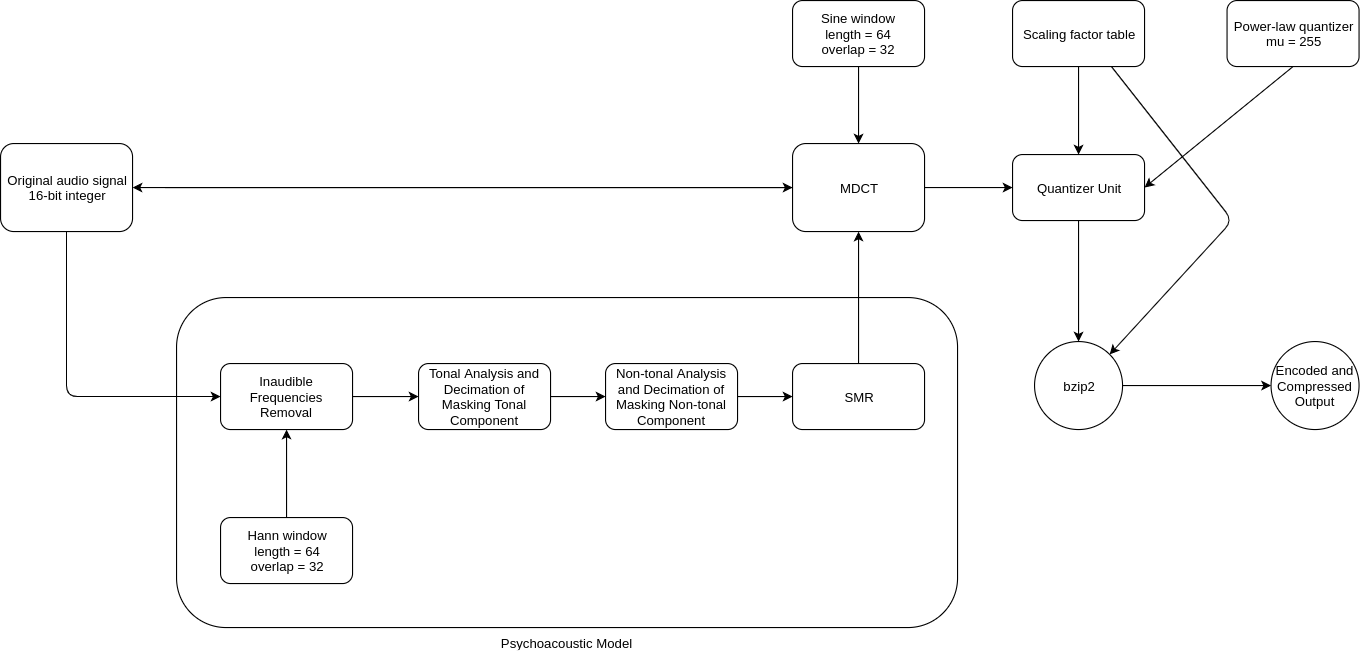
\includegraphics[width=1\linewidth]{flow_diagram_codec}
		\caption{}
		\label{fig:flowdiagramcodec}
	\end{figure*}
	
	\section{Modified Discrete Cosine Transform}
	
	MDCT is a lossless compression algorithm \cite{b1}, based on the type-IV DCT, whose coefficients are described by $C_M$:
	
	\begin{equation}
	C_M = cos[\frac{\pi}{M}(k + \frac{1}{2})(n + \frac{1}{2})]_{k,n=0,1...M-1}
	\label{eq1}
	\end{equation}
	
	However, in MDCT, the coefficient matrix $E_{2M}$ is:
	
	\begin{equation}
	E_{2M} = cos[\frac{\pi}{M}(k + \frac{1}{2})(n + \frac{M}{2} + \frac{1}{2})]_{k=0,1...M-1, n=0,1...2M-1}
	\label{eq2}
	\end{equation}
	
	which is the same as:
	
	\begin{equation}
	E_{2M} = cos[\frac{\pi}{M}(k + \frac{1}{2})(n + \frac{1}{2})]_{k=0,1...M-1, n=\frac{M}{2},...,\frac{M}{2}+2M-1}
	\label{eq3}
	\end{equation}
	
	It is apparent that Equation \ref{eq3} is very similar to Equation \ref{eq1}. Hence, Equation \ref{eq3} can be rewritten as:
	
	\begin{equation}
	E_{2M} = C_M[I_M -J_M -I_M J_M]P\left[\begin{matrix}I_{2M} \\ 0\end{matrix}\right]
	\label{eq4}
	\end{equation}
	
	where $I_{M}$ is the identity matrix $M\times M$ and $J_{M}$ is the negative of $I_M$. For:
	
	$$Q = [I_M -J_M -I_M J_M]$$
	
	and
	
	$$R = QP\left[\begin{matrix}I_{2M} \\ 0\end{matrix}\right]$$
	
	then, the coefficients of the MDCT, $E_{2M} = X$, are:
	
	\begin{equation}
	X = C_MRx
	\label{eq5}
	\end{equation}
	
	Hence, the original signal, $\hat{x}$, can be re-synthesized from $X$ by:
	
	\begin{equation}
	\hat{x}=(C_MRx)^TX = (R^TC_M^T)X = (R^TC_M^T)(C_MRx)
	\label{eq6}
	\end{equation}
	
	the product $C_M^TC_M$ is $I_M$ but $R^TR$ is not $I_M$
	
	\begin{equation}
	\hat{x}=(R^TRC_M^TC_M)x = (R^TRI_M)x
	\label{eq7}
	\end{equation}
	
	In order to make $\hat{x} = x$, $R^TR$ must be $I_M$. This can be done by having a window overlap of half the window size. All the time-domain-aliasing (TDAC) produced by the overlap will be cancelled out, leaving the transform with completely unaliased reconstruction \cite{b2}.
	
	The code for MDCT and IMDCT used for this codec is written by Zafar Rafii, and can be found at \url{https://github.com/zafarrafii/Z/blob/master/z.py}
	
	\newpage
	\section{Psychoacoustic Model}
	
	The psychoacoustic model implemented in this codec is a simpler version described in the paper \cite{b3} written by Joebert S. Jacaba, Dept. Mathematics, College of Science, University of The Philippines, Diliman, Quezon City: \textit{Audio Compression using Modified Discrete Cosine Transform: The MP3 Coding Standard}. Available at: \url{https://www.mp3-tech.org/programmer/docs/jacaba_main.pdf}
	
	The model consists of 3 parts: 
	\begin{itemize}
		\item Inaudible frequencies removal
		\item Tonal analysis and decimation of masking tonal component
		\item Non-tonal analysis and decimation of masking non-tonal component
		\item Signal-to-mask ratio
	\end{itemize}
	
	\subsection{Inaudible Frequencies Removal}
	
	The first step involves calculating the Power Density Spectrum $P(k,i)$ of the audio signal for time frame $i$ and a frequency $k$. The Short-Time Fourier Transform (STFT) is performed on the signal with a Hanning window, in which the length is $N$, and the hop length is $N/2$. Then:
	
	\begin{equation}
	P(k,i) = PN + log_{10}(STFT(x)^2) (dB), 0 \le k \le N/2
	\label{eq8}
	\end{equation}
	
	where PN is a Power Normalization term, so that the maximum value of $P(k,i)$ is 96dB. With a window length of 64 and hop length of 32, k runs from 0 to 32, which correspond to the 33 frequency bands. The first band will be ignored because the frequencies in this band have very low energy, and the MDCT with the same window only produces the upper 32 bands.
	
	Each of these frequency bands will be assigned a frequency number that is the maximum frequency of the band $f(k)$. For all frequencies in $f(k)$, the critical band rate, or bark unit can be extracted as $b(k)$, and the absolute threshold of hearing can be calculated as $ath(k)$:
	
	\begin{equation}
	b(k) = 13 tan^{-1}(0.00076f(k)) + 3.5 tan^{-1}((\frac{f(k)}{7500})^2)
	\label{eq9}
	\end{equation}
	
	\begin{equation}
	\begin{split}
	ath(k) = 3.64(\frac{f}{1000})^{-0.8} - 6.5exp(-0.6(\frac{f}{1000} - 3.3)^2) \\
	+ 0.001(\frac{f}{1000})^4
	\label{eq10}
	\end{split}
	\end{equation}
	
	Hence, for all frames and frequencies $i, k$, if $P(k,i) < ath(k)$, then the position $(k,i)$ are marked to be decimated later in the MDCT.
	
	\subsection{Tonal Analysis and Decimation of Masking Tonal Component}
	
	Using the same power density spectrogram $P(k,i)$, the power local "peaks" can be found for every frame $i$. A spectral line is a peak when:
	$$P(k,i) > P(k-1,i)$$ 
	and 
	$$P(k,i) \ge P(k+1,i)$$
	
	Hence, a peak at position $(k,i)$ is a tonal component if:
	
	$$P(k,i) - P(k+j,i) \ge 7 dB, j=[2,-2]$$ 
	
	Finally, the sound pressure level (SPL) of the tonal component $P_{TN}$ is:
	
	$$P_{TN}(k,i) = P(k-1,i) + P(k,i) + P(k+1,i)$$
	
	From the constructed list of the tonal components and their SPLs, mark all positions $(k,i)$ such that: if $|b(k_1,i) - b(k_2,i)| < 0.5$, then $(k,i)$ is the position of the tonal component with smaller SPL because this tonal component will be "masked" by the one with higher SPL.
	
	\subsection{Non-tonal Analysis and Decimation of Masking Non-tonal Component}
	
	The non-tonal components can be calculated as the "subtracted image" between the original power density spectrum and the tonal component map. For each non-tonal components $P_{NT}$, group them into the 26 critical bands, $b(k)$. Then, the non-tonal component corresponding to each critical band in each frame $i$ will have the SPL equals to the sum of the power of all the frequencies $k$ in that band, and the position equals to the geometric average of all the the frequencies $k$ in that band. 
	
	From this constructed list of all the major non-tonal components, do the same marking process as for the tonal components. The marked positions will be decimated later in the MDCT.
	
	\subsection{Signal-to-mask Ratio}
	
	Although the signal-to-mask ratio (SMR) will not be calculated for this codec due to complexity, it is a vital process because the SMR for each band (out of 32) determines the scaling factor for that band. This scaling factor determines the importance of the band towards the reconstruction of the signal, which creates the non-uniform quantization of the bands in the MDCT. Instead, a fixed, empirically determined scaling factor will be assigned to the MDCT's bands.
	
	\newpage
	
	\section{Quantizer Unit}
	
	The quantization steps begin with define the scaling factors table for the 32 bands resulting from the MDCT. The table is as follow:
	
	% Insert table of scalling factors
	\begin{table}[htbp]
		\caption{Table of scaling factors for each bands of the MDCT}
		\begin{center}
			\begin{tabular}{|c|c|c|c|c|c|}
				\hline
				\textbf{Band \#}&\textbf{Scale}&\textbf{Band \#}&\textbf{Scale}&\textbf{Band \#}&\textbf{Scale} \\
				\hline
				0 & 19 & 8 & 32 & 16 & 32 \\
				\hline
				1 & 19 & 9 & 20 & 17 & 32 \\
				\hline
				2 & 19 & 10 & 23 & 18 & 32 \\
				\hline
				3 & 19 & 11 & 23 & 19 & 32 \\
				\hline
				4 & 19 & 12 & 23 & 20 & 32 \\
				\hline
				5 & 21 & 13 & 32 & 21 & 32 \\
				\hline
				6 & 21 & 14 & 32 & ... & ... \\
				\hline
				7 & 21 & 15 & 32 & 31 & 32 \\
				\hline
			\end{tabular}
			\label{tab1}
		\end{center}
	\end{table}
	
	After the scales are defined, each band of the MDCT is passed through the $\mu$-law (or power law) quantizer with $\mu = 255$ so that all the numbers are in between -1 and 1. Then, depending in which bands these numbers are in, they are divided by $2^{\text{scale of the band}}$. Finally, all numbers are quantized again from 32-bit floats to 16-bit floats. 
	
	The quantized MDCT, along with the table of scaling factors are encoded as a byte-string and zipped using bzip2 algorithm, which includes Huffman coding. 
	
	This zipped file is the output of the compression algorithm in this paper.
	
	\section{Decompression}
	
	Taking the zipped file as an input, the decompression algorithm unzips the file, multiplies each row of the quantized MDCT with $2^{\text{scale of the band}}$, inverts power-law quantization, and inverts MDCT on that output to get back the original signal.
	
	\section{Results}
	Many literatures have cited the compression ratio of MP3 is 11:1 at 128 kbit/s (CD quality) \cite{b4}. If the input audio format is 16-bit integers, then SNR of CD Quality is estimated with:
	
	\begin{equation}
	SQNR = 20log_{10}(2^{16}) \approx 24.08 dB
	\end{equation}
	
	where SQNR is the signal-to-quantization-noise ratio \cite{b5}. 
	
	The codec in this paper can deliver different compression ratio by modifying the scaling factors table above. With the one listed in this paper, however, the average compression ratio is 7.96 and the average SNR is 23.85. The testing audio signals are 5 different songs: Taxman by The Beatles, Another Brick In The Wall by Pink Floyd, Stairway To Heaven by Led Zeppelin, Baby by Justin Bieber, and On My Way by Farruko, Alan Walker, Sabrina Carpenter. 
	
	Without the quantizer unit (only MDCT and PAM at work), the average compression ratio is 2.13 and the average SNR is 79.95. 
	
	The quantizer unit reduces the dynamic range of the signal, which muffles the audio and create popping sounds at very high frequencies. 
	
	Overall, the codec works as expected. If the psychoacoustic unit can be improved to include SMR, which replaces the static scaling factors, the decompressed output can have much higher SNR (40-60 dB) although the compression ratio may suffer as a result.
	
	\begin{thebibliography}{00}
		\bibitem{b1} Ochoa-Domínguez, Humberto, and K. R. Rao. “The Modified Discrete Cosine Transform.” Discrete Cosine Transform, 2019, pp. 113–132., doi:10.1201/9780203729854-5.
		\bibitem{b2} Werner, et al. “Experimenting with Lapped Transforms in Numerical Computation Libraries Using Polyphase Matrices and Strided Memory Views.” Audio Engineering Society, Audio Engineering Society, 10 Mar. 2019, www.aes.org/e-lib/browse.cfm?elib=20381.
		\bibitem{b3} Jacaba, Joebert S. “Using Modified Discrete Cosine Transform: The MP3 Coding Stan.” CORE, 1 Jan. 1970, core.ac.uk/display/20736021.
		\bibitem{b4} Woon-Seng Gan; Sen-Maw Kuo (2007). Embedded signal processing with the Micro Signal Architecture. Wiley-IEEE Press. p. 382. ISBN 978-0-471-73841-1.
		\bibitem{b5} B.P.Lathi , Modern Digital and Analog Communication Systems (3rd edition), Oxford University Press, 1998
		
	\end{thebibliography}
	
\end{document}
